\documentclass[dvisvgm,border=2pt]{standalone}
% Shared by every figure. Two colours only: black becomes the text colour of
% whatever theme the app is in, and `accent` becomes the brand — see
% scripts/build-figures.mjs. Everything else is done with opacity.
\usepackage{amsmath}
\usepackage{amssymb}
\usepackage{tikz}
\usepackage{pgfplots}
\pgfplotsset{compat=1.18}
\usetikzlibrary{arrows.meta,positioning,calc,backgrounds,fit,patterns.meta}
\definecolor{accent}{RGB}{255,0,255}
\pgfplotsset{
  every axis/.append style={
    axis lines=left,
    axis line style={draw opacity=0.35},
    tick style={draw opacity=0.35},
    tick label style={font=\scriptsize,opacity=0.7},
    label style={font=\scriptsize,opacity=0.7},
    legend style={draw=none,fill=none,font=\scriptsize},
    every axis plot/.append style={line width=0.7pt},
  },
}
\tikzset{
  every picture/.style={font=\scriptsize},
  faint/.style={opacity=0.3},
  quiet/.style={opacity=0.55},
  box/.style={draw,opacity=0.35,rounded corners=2pt,inner sep=4pt},
  hot/.style={accent},
}

\begin{document}
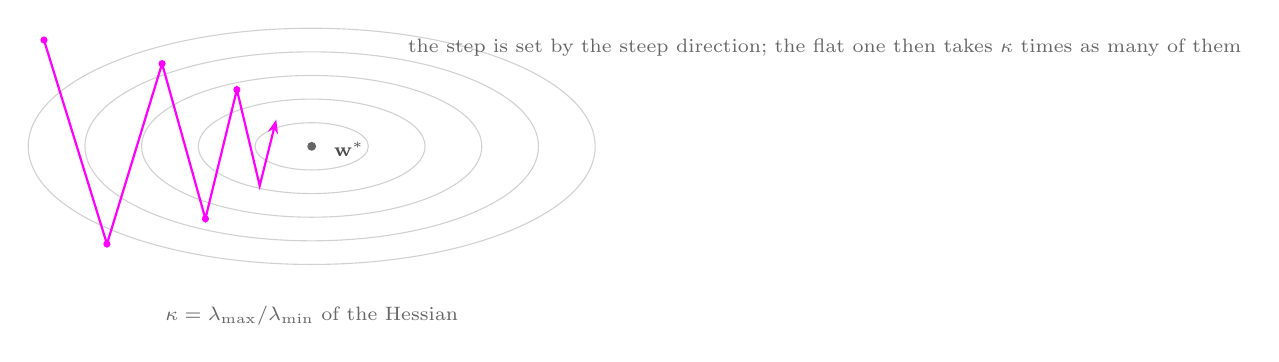
\begin{tikzpicture}[every node/.style={font=\scriptsize}]
  \foreach \k in {1,...,5}
    \draw[opacity=0.18] (0,0) ellipse ({\k*0.72} and {\k*0.3});
  \fill[opacity=0.6] (0,0) circle (1.6pt);
  \node[opacity=0.7,anchor=west] at (0.16,-0.04) {$\mathbf{w}^{*}$};
  \draw[accent,line width=0.8pt,-{Stealth[length=5pt]}]
    (-3.4,1.35) -- (-2.6,-1.24) -- (-1.9,1.05) -- (-1.35,-0.92)
    -- (-0.95,0.72) -- (-0.66,-0.5) -- (-0.45,0.34);
  \foreach \p in {(-3.4,1.35),(-2.6,-1.24),(-1.9,1.05),(-1.35,-0.92),(-0.95,0.72)}
    \fill[accent] \p circle (1.3pt);
  \node[opacity=0.6,align=left,anchor=west] at (1.1,1.25)
    {the step is set by the\ steep direction; the flat\ one then takes $\kappa$ times\ as many of them};
  \node[opacity=0.6,anchor=north] at (0,-1.9) {$\kappa=\lambda_{\max}/\lambda_{\min}$ of the Hessian};
\end{tikzpicture}
\end{document}
